\documentclass{article}
\usepackage{titlesec}
\usepackage{graphicx}
\graphicspath{ {./Images/} }
\usepackage{xcolor}
\usepackage{listings}
\usepackage{wrapfig}
\usepackage{subcaption}
\usepackage{float}

\definecolor{mGreen}{rgb}{0,0.6,0}
\definecolor{mGray}{rgb}{0.5,0.5,0.5}
\definecolor{mPurple}{rgb}{0.58,0,0.82}
\definecolor{backgroundColour}{rgb}{0.95,0.95,0.92}

\lstdefinestyle{pythonStyle}{
    backgroundcolor=\color{backgroundColour},   
    commentstyle=\color{mGreen},
    keywordstyle=\color{magenta},
    numberstyle=\tiny\color{mGray},
    stringstyle=\color{mPurple},
    basicstyle=\footnotesize,
    breakatwhitespace=false,         
    breaklines=true,                 
    captionpos=b,                    
    keepspaces=true,                 
    numbers=left,                    
    numbersep=5pt,                  
    showspaces=false,                
    showstringspaces=false,
    showtabs=false,                  
    tabsize=2,
    language=python
}
\author{Juan Alejandro Bernal, Orlando Hernandez}
\title{\textbf{Informe Aplicaci\'on Solucionador De Sudokus}}
\date{\today}

\begin{document}
\maketitle
\section{Problema a resolver}
\subsection{Introducción}
El sudoku es un juego matemático inventado en 1970,  
recibió muy poca atención del publico en sus inicios, pero en 
la decada de 1984 recibió mucha atención en japón, finalmente
en el 2005 tomo importancia internacional ya que empezaron
a ser publicados en periódicos.
\subsection{Descripción}
Un sudoku es una cuadricula de 9 x 9  dividida en subcuadrillas
de 3 x 3, en total hay 81 casillas. El objetivo es rellenar las
81 casillas, teniendo en cuenta que algunas casillas ya están rellenadas
de ante mano. La solución de un sudoku siempre es un cuadrado latino con la única 
diferencia que en cada subcuadrillas no hayan números repetidos.
\subsection{Dificultad}
La dificultad de un sudoku depende del número de soluciones posibles que hayan 
dependiendo de los valores que están ya dispuestos en las celdas. El matemático Gary
McGuire a demostrado que el mínimo número de cifras para conseguir un sudoku con una única solución es de 17 cifras.
Esto se da por que dadas las condiciones del cuadrado latino y que los números no se pueden
repetir en subcuadrillas, las posibilidades que existen para poner números en lugares equivocados
es muy alta. 
\section{Solución}
Por la alta dificultad que pueden tener algunos sudokus hemos diseñado una aplicación que se
encarga de recibir un sudoku y devolver una solución. A diferencia de la mayoría
de programas que existen capaces de solucionar sudokus en la actualidad, esta aplicación
es capaz de hacerlo con números que el jugador ya haya ingresado, y asi encontrar todas las
posibles soluciones desde el punto en el que se encuentre parado.
Haciendo uso de técnicas de reconocimiento de patrones y visión artificial. 
Con la idea de hacerlo mas sencillo de usar se creo una interface movil
haciendo uso del kit de desarrollo open-source "flutter" de Google. 
\subsection{Pasos para reproducir la solución}
\subsubsection{instalacion de Dependencias}
\subsubsection{Manual}
\subsection{Explicación técnica}
Aquí empezaremos a explicar como funciona la aplicación, que técnicas de inteligencia artificial se utilizaron y el algoritmo usado para la solución del sudoku.
\subsubsection{Visión por computadora}
El algoritmo utilizado para encontrar el contorno de las imágenes sigue el contorno binario haciendo
un análisis topologico de la imagen digital, según \cite{test} se sigue un patrón de color o intensidad
la cual la computadora sigue como patrón de la siguiente manera:
\begin{figure}[H]
\caption{Ejemplo de imágenes en visión artificial}
\centering
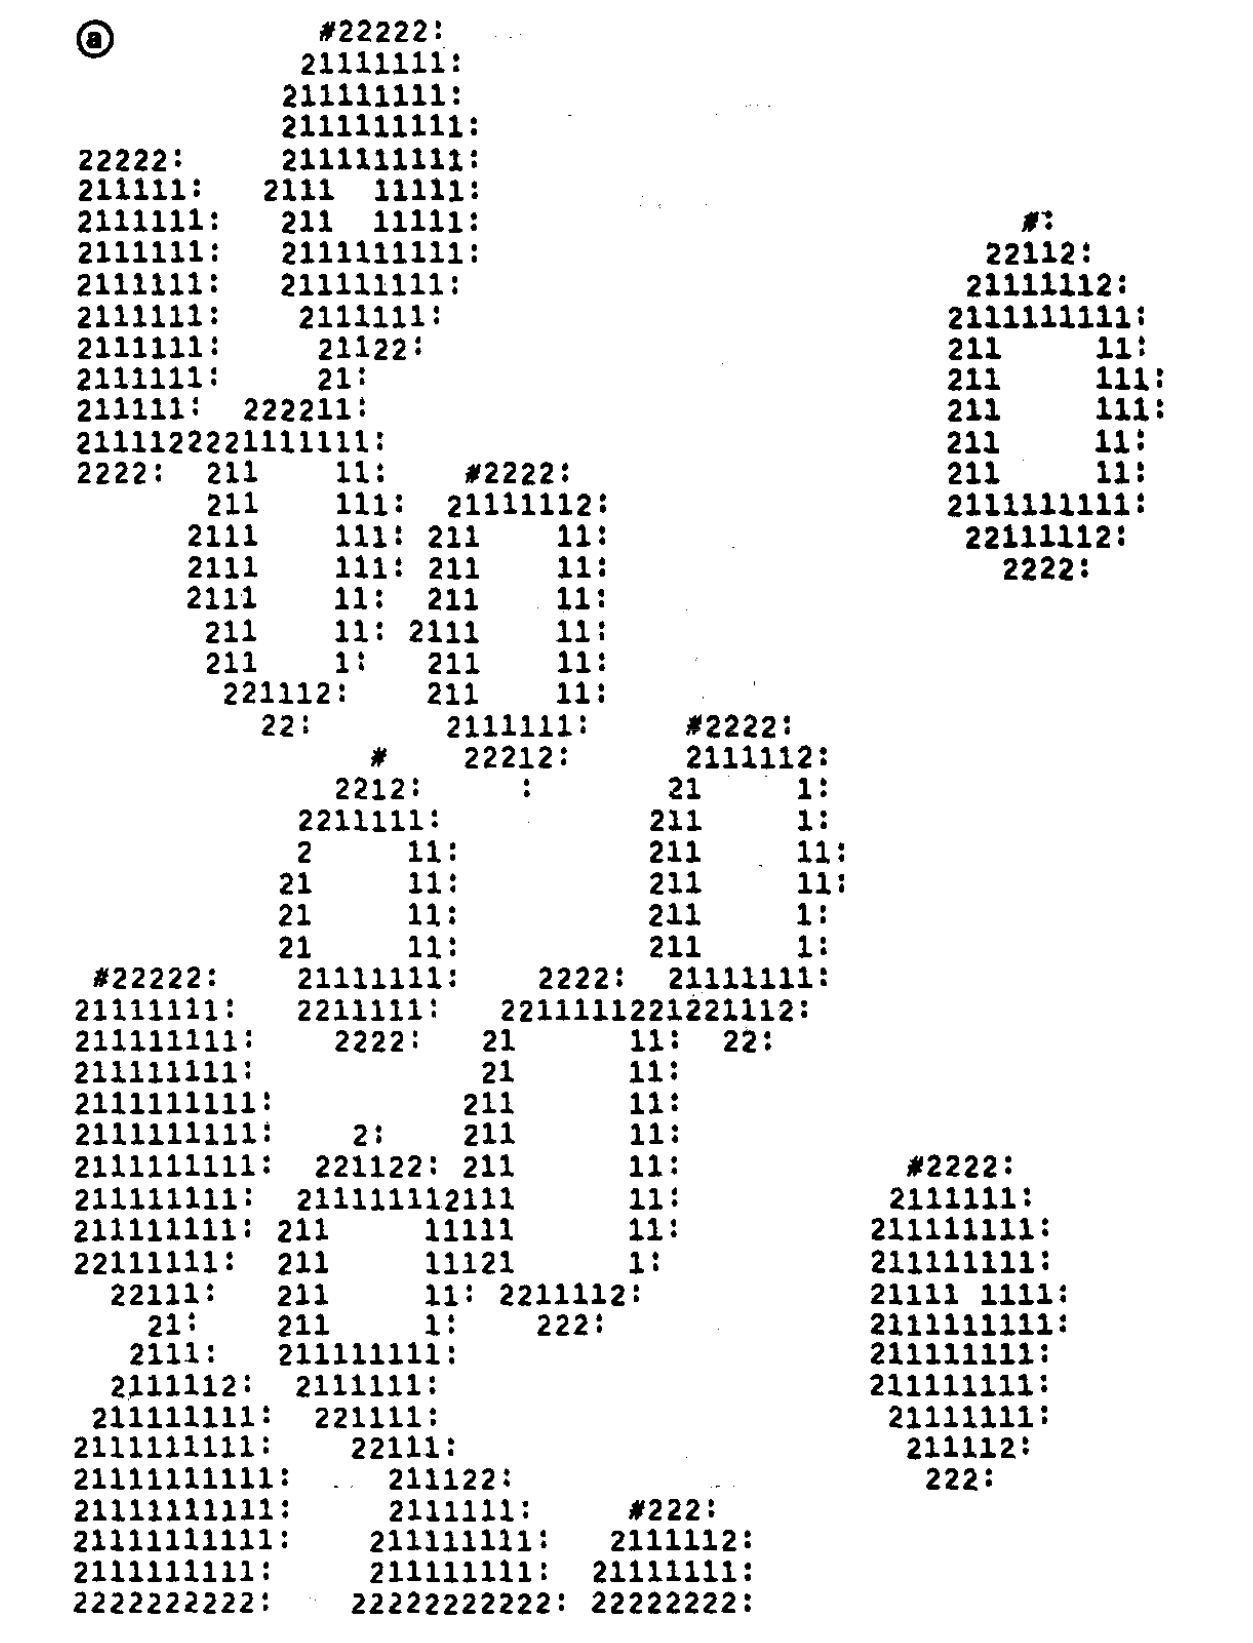
\includegraphics[scale=.15]{a}
\end{figure}
\begin{wrapfigure}{l}{0.4\textwidth}
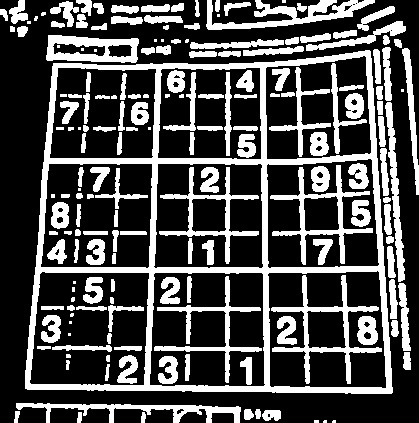
\includegraphics[width=1\linewidth]{filtro}
\caption{Filtro aplicado a un sudoku}
\end{wrapfigure}
Como se puede observar en la imagen los contornos empiezan en el símbolo \# y continúan donde están marcados los
:. El uso de filtros hace que este algoritmo reconozca estos patrones de manera mas sencilla, en especial el 
pasar la imagen a un estado binario de forma que quede asi:

Haciendo uso de esto podemos conseguir todos los contornos de una imagen de sudoku, al conseguir los contornos
los procesamos haciendo uso del algoritmo de Ramer-Douglas Peucker \cite{ramer} la cual (en resumen) aproxima los puntos
a lineas, las cuales consideraremos como lados, el cual nos permite encontrar todos los cuadrados del sudoku.
Pero como primera instancia debemos de encontrar el cuadrado mas grande, es decir el mas externo.
\vspace{.3cm}
\begin{lstlisting}[style=pythonStyle]
for contour in contours:
         perimeter = cv2.arcLength(contour,True) # largo del contour
         approx = cv2.approxPolyDP(contour, 0.02*perimeter , True) # funcion Ramer, 0.02 es una constante
         if len(approx) == 4: # si es un cuadrado
             if perimeter > maxPerimeter: # para conseguir el contorno mas grande
                 maxPerimeter = perimeter
                 big_square = approx
    return big_square
\end{lstlisting}
Una vez encontrado el contorno mas grande nos queda un arreglo con 4 tuplas las cuales representan los puntos
en las esquinas, los cuales usaremos para poder hacer una transformación de perspectiva a la imagen, ya que
como las fotos pueden ser tomadas en ángulos extraños, se necesita arreglar la perspectiva para que ayude a la
detección de números después.

\begin{figure}[H]
\centering
\begin{subfigure}{.5\textwidth}
  \centering
  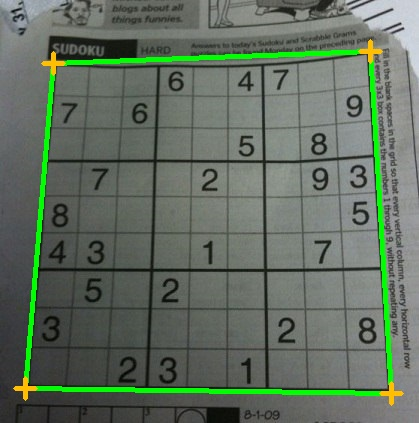
\includegraphics[width=.6\linewidth]{esquinas}
  \caption{Transformacion}
  \label{fig:sub1}
\end{subfigure}%
\begin{subfigure}{.5\textwidth}
  \centering
  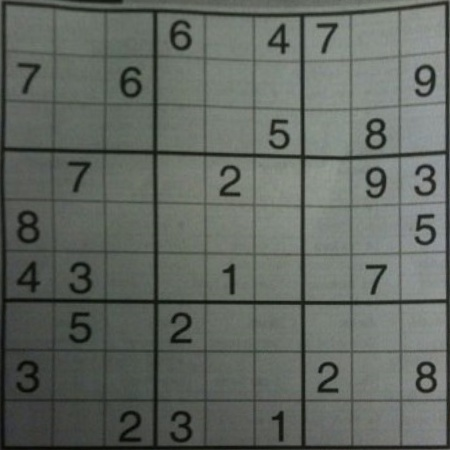
\includegraphics[width=.6\linewidth]{transformada}
  \caption{Esquinas encontradas}
  \label{fig:sub2}
\end{subfigure}
\caption{Procesamiento de imagen}
\label{fig:test}
\end{figure}

finalmente dividimos el sudoku en sus lineas interiores  para poder conseguir
un arreglo de subcuadros, los cuales usaremos para hacer el reconocimiento de 
dígitos

\begin{figure}[H]
\caption{Arreglo de subcuadros}
\centering
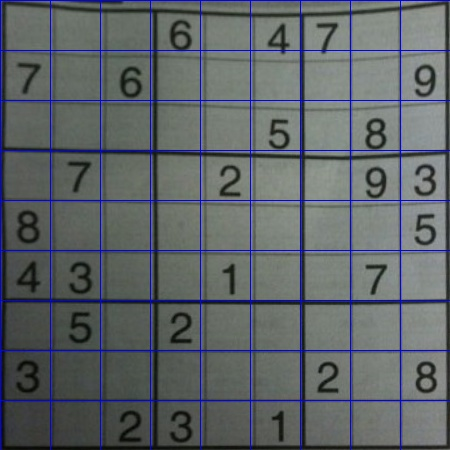
\includegraphics[width=.8\textwidth]{squares}
\end{figure}
% \begin{figure}[h]
% \centering
% \caption{Esquinas de un sudoku}
% 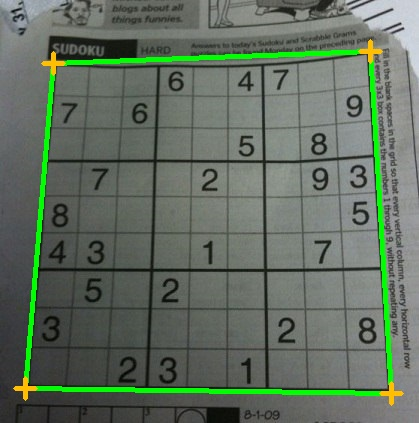
\includegraphics[scale=.3]{esquinas}
% \end{figure}

\subsubsection{Reconocimiento de dígitos}
\subsubsection{Backtracking}
\section{Resultados}
\bibliographystyle{ieeetr}
\bibliography{uni}
    
\end{document}











